%%
%% ****** Generated 24.03.23 by LJM TeX-constructor******
%%
\documentclass{article}

\usepackage{amssymb}
\usepackage{amsfonts}
\usepackage[tbtags]{amsmath}
\usepackage{amscd}
\usepackage{amsthm}			% Продвинутая математика
\usepackage{mathtext}
\usepackage{cmap}
\usepackage[T2A]{fontenc}
\usepackage[utf8]{inputenc}			% cp1251
\usepackage[english, russian]{babel}
%\usepackage{literat}
\usepackage{pifont}
\usepackage{bm}
\usepackage{array}			% Ширина столбиков в массиве
\usepackage{dcolumn}
\usepackage{hhline}
\usepackage{multirow}
\usepackage{graphicx}
\usepackage{rotating}
\usepackage{calc}
\usepackage{tabularx}
\usepackage{afterpage}
\usepackage{ifthen}
\usepackage{caption2}
\usepackage{substr}
\usepackage[mathscr]{eucal}  %% My addition
\usepackage{mathrsfs}        %% My addition
\usepackage{hypbmsec}        %% My addition
\usepackage{latexsym}        %% My addition
\usepackage{xypic}           %% My addition
\RequirePackage{soul}
\RequirePackage{verbatim}    %% My addition
\RequirePackage{chapterbib}
\RequirePackage{enumerate}


\usepackage[shortcuts]{extdash}
\usepackage{ragged2e}
\usepackage{etoolbox}
\usepackage{lipsum}

%\usepackage{flafter}
\usepackage[section,above,below]{placeins}

\usepackage{indentfirst}
\usepackage[a4paper, top=20mm, left=30mm, right=20mm, bottom=25mm]{geometry}


\setcounter{page}{1}

\begin{document}
\title{Применение методов машинного обучения для восстановления свойств подвижности и сжимаемости элемента нефтяного месторождения} % for running heads
\author{Kosyakov} % for running heads
\author{Legostaev}

%\noaffiliation % If the author does not specify a place of work.

%\firstcollaboration{(Submitted by ) } % Add if you know submitter.
%\lastcollaboration{ }


\begin{abstract} % You shouldn't use formulas and citations in the abstract.
В нефтяной отрасли наблюдается заметная тенденция к прокси-моделированию различных уровней сложности для выполнения оперативных прогнозных расчетов, в частности, к методам машинного обучения, которые активно развиваются в контексте цифровизации и интеллектуализации производственных процессов. В этой статье на примере элемента разработки модели синтетического нефтяного пласта мы представляем подход к совместному использованию физически значимой модели потока жидкости и методов машинного обучения для решения задач адаптации и прогнозирования. Особенностью рассматриваемой синтетической модели является наличие выраженной зональной неоднородности поля проницаемости. В рамках предложенного подхода была использована упрощенная по сравнению с исходной формулировкой модель однофазной фильтрации, которая была сопоставлена с историей путем восстановления поля параметров фильтрации коллектора с использованием сети радиальных базисных функций. На основе реконструированного месторождения были рассчитаны коэффициенты связи между скважинами, которые качественно и количественно соответствуют истинной связи скважин. Для оценки прогностических свойств моделей фактический набор данных был разделен на обучающие и тестовые интервалы.
\end{abstract}

\textbf{Keywords}:flow through porous medium, reservoir mathematical simulation, inverse problem, adjoint problem, machine learning, radial basis functions% Include keywords separeted by comma.

\maketitle

% Text of article starts here.
\section{INTRODUCTION}

В настоящее время в нефтедобывающей отрасли, наряду с использованием традиционных гидродинамических моделей, широко применяется использование упрощённых прокси-моделей. Использование упрощённых моделей позволяет сократить вычислительные затраты, а также снизить требования к качеству и полноте исходных данных. Развитие и применение прокси-моделирования для обратных и оптимизационных задач является актуальным, так как они являются самыми ресурсоёмкими задачами. Помимо физически содержательных моделей (материальный баланс \cite{mus1}, супер элементы, CRM \cite{bek}, линии тока \cite{pot} и т.д.), развиваются подходы, основанные на применении методов машинного обучения \cite{tem}, \cite{uma}. Например, рекуррентные нейронные сети получили применение в области прогнозирования временных рядов и, в частности, режимов работы скважин. Однако, применение подходов, основанных только на методах машинного обучения, в качестве прогнозирующих моделей не может гарантировать получения верного с точки зрения физики процесса результата. Совместное использование физически содержательной модели и методов машинного обучения позволяет избегать проблем подобного рода \cite{kos2}.

На рисунке \ref{fig:schime1} представлена общая схема используемого подхода. Алгоритм работы заключается в том, что методы машинного обучения объединяются с физически содержательной фильтрационной моделью, которая используется в качестве одного из слоёв полученной “гибридной” нейронной сети. При данном подходе на вход блока машинного обучения подается одна часть данных «input ML», рассчитываются значения «output ML», которые вместе со второй частью данных «input Flow» выступают в качестве входа для расчета «Flow». Для настройки параметров модели «ML» используются результаты решения сопряженной задачи («Flow derivative»), которые позволяют рассчитать градиент для фильтрационной части. Расчёт градиента для элементов МО выполняется с помощью стандартной процедуры обратного распространения ошибки. Для ФМ расчёт градиента является отдельной трудоёмкой задачей, вычислительная сложность которой, как правило, сопоставима или превосходит сложность прямого расчёт ФМ. Расчёт градиента для ФМ вынесен в отдельный блок решения сопряжённой задачи.

\begin{figure}
	\centering
	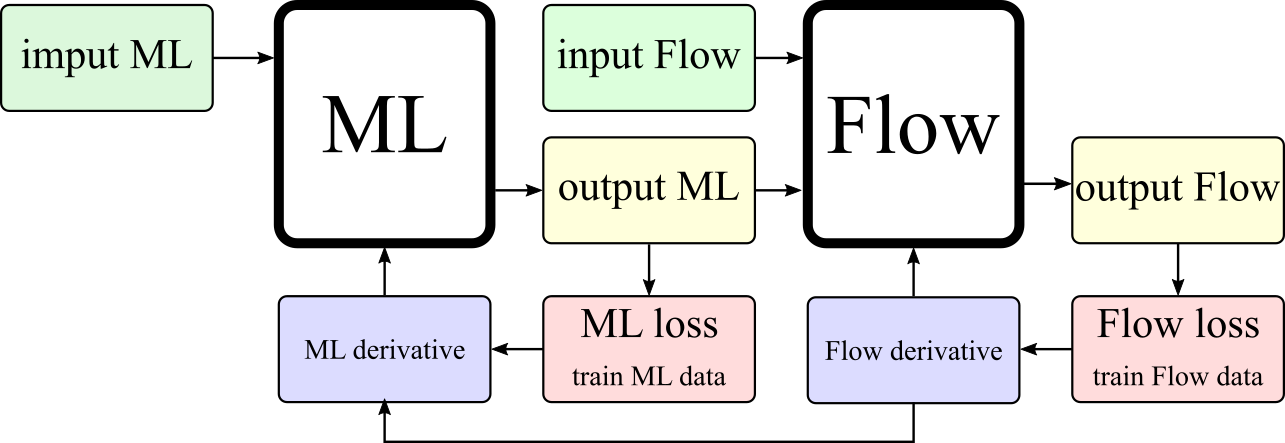
\includegraphics[width=0.7\linewidth]{fig0}
	\caption{A calculation scheme for the proposed algorithm for the combined use of machine learning and a single-phase flow model.}
	\label{fig:schime1}
\end{figure}

Целью настоящей работы является развитие инструментов прокси-моделирования на основе теории фильтрации и элементов машинного обучения. Задача восстановления фильтрационно-ёмкостных параметров пластовой системы в межскважинном пространстве при помощи сети радиально-базисных функций была решена путем адаптации фильтрационной модели на известные значения пластового давления при заданных расходах жидкости на скважинах. Для контроля прогностических свойств моделей проведено разбиение моделируемого периода разработки на обучающий и тестовый интервалы.

\section{Mathematical Model}

\subsection{Single-phase flow model}
Для решения этой задачи в качестве модели фильтрации была использована двумерная математическая модель однофазного течения
слабосжимаемой жидкости:

\begin{equation} \label{fil}
	\triangledown \cdot \left[\frac{k}{\mu}\triangledown P \right] = \beta h\frac{dP}{dt} + \delta_{l}(x,y),
\end{equation}

\begin{equation} \label{bc}
	\delta_{i}(x,y)  = \left\{\begin{array}{crl}
		0, \;\mbox{if}\;(x,y) \notin\ \Gamma_{in}\cup\Gamma_{out},\\
		q_{i\:k}, \;\mbox{if}\;(x,y) \in \Gamma_{in},\\
		q_{i\:aq}, \;\mbox{if}\;(x,y) \in \Gamma_{out},
	\end{array}\right. \quad i = l,w.
\end{equation}
Closing ratios:
\begin{equation} \label{kr}
P = P_0\mbox{,\quad \mbox{if} $t=0$},
\end{equation}
where $k$ is permeability, $P$ is reservoir pressure, $\beta$ is
effective compressibility, $h$ is effective thickness, subscript $i$ denotes $l$ -- liquid
(water and oil), $q_k$ is fluid flow rate in $k$th well, $\Gamma_{in}$
is set of coordinates of sources/drain (wells), $\Gamma_{out}$ is
outer boundary, $P_0$ is reservoir pressure at the initial time $t=0$, $q_{aq}$ is specific fluid flow rate through the outer boundary, which can be written as:
\begin{equation*} \label{qaq}
	q_{i\:aq} = T_a(P_{a} - P|_{\Gamma_{out}}),
\end{equation*}
where $P_a$ is on the aquifer ($P_a = P_0$), $T_a$ is
aquifer boundary transmissibility (includes aquifer productivity factor). The goal of the inverse problem is to find the reservior permeability $k = k(x,y)$ and effective compressibility $\beta = \beta(x,y)$ at which the calculated values of reservoir pressure and water flow rate on the wells will satisfactorily coincide with the initial values.

\subsection{RBF}

Получение значений $k(x,y)$ и $\beta(x,y)$ возможно различными способами, например интерполяция и экстраполяция измеренных значений вблизи скважин в область межскваженного пространства. В настоящей работе предлагается получение искомых значений при использовании модели машинного обучения. В качестве модели машинного обучения была выбрана двухслойная нейронная сеть, состоящая из слоя радиально-базисных функций (РБФ) и полносвязного слоя. Слой РБФ определяет влияние каждого базиса на выбранную точку пространства.

При решении обратной задачи удобнее от проницаемости $k$ перейти к общей подвижности $\lambda$, при помощи этого параметра можно комплексно учесть множество фильтрационных параметров влияющих на структуру фильтрационных потоков (вязкость, относительные фазовые проницаемости и т.д.). 
Поля общей подвижности $\lambda$ и эффективной сжимаемости $\beta$ рассматриваются в виде функциональной зависимости $\lambda(\mathbf{x})$ и $\beta(\mathbf{x})$, где  $\mathbf{x}$ – вектор пространственных координат. В качестве зависимости использована сеть радиально базисных функций.

\begin{eqnarray}\label{rbf}
	f_i(\mathbf{x}) = exp \left(\frac{-\lVert \mathbf{x} - \mathbf{c_f}_i \rVert^2}{\epsilon_{fi}^2}\right), \quad
	g_i(\mathbf{x}) = exp \left(\frac{-\lVert \mathbf{x} - \mathbf{c_g}_i \rVert^2}{\epsilon_{gi}^2}\right),
\end{eqnarray}

\begin{eqnarray}
	\lambda(\mathbf{x}) = w_{fi}f_i + b_h, \quad
	\beta(\mathbf{x}) = w_{gi}g_i + b_g,
\end{eqnarray}
где $\mathbf{x}$ – координаты расчетных узлов,  $\mathbf{c_f}_i$ и $\mathbf{c_g}_i$– положение базисов, $\epsilon_{fi}$ и $\epsilon_{gi}$– ширина базисов, $w_{fi}$ и $w_{gi}$ – веса базисов, $b_f$ и $b_g$ – свободный член. Параметры сети радиально базисных функций $\mathbf{c}_i$, $\epsilon_i$, $w_i$, $b$  настраиваются в процессе адаптации однофазной фильтрационной модели.

\subsection{INVERSE PROBLEM}

Обратная задача решается в оптимизационной постановке, которая заключается в минимизации целевой функции $J$.
Целевая функция может быть записана в виде суммы слагаемых, каждое из которых является произведением функции, характеризующей отклонение
вычисленных значений от контрольных, и весового коэффициента для соответствующего типа переменной. В качестве меры отклонения была выбрана среднеквадратичная ошибка (MSE).
\begin{equation} \label{mse}
	J=\frac{w_p}{N_p}\sum_{i=1}^{N_p}{\left(p_c^i-p_f^i\right)^2}+
	\frac{w_{\lambda}}{N_\lambda}\sum_{i=1}^{N_\lambda}{\left(\Delta\lambda^i  \right)^2}+
	\frac{w_{\beta}}{N_\beta}\sum_{i=1}^{N_\beta}{\left(\Delta\beta^i  \right)^2},
\end{equation}
\begin{equation}
		\Delta\lambda^i  = \left\{\begin{array}{crl}
		\lambda^i - \hat{\lambda}_r, \quad \;\mbox{if}\; \lambda^i \ge \hat{\lambda}_r\\
		0,\quad \;\mbox{if}\; \hat{\lambda}_l < \lambda^i < \hat{\lambda}_r\\
		\lambda^i - \hat{\lambda}_l, \quad \;\mbox{if}\;\lambda^i \le \hat{\lambda}_l,
	\end{array}\right.
		\quad
		\Delta\beta^i  = \left\{\begin{array}{crl}
		\beta^i - \hat{\beta}_r, \quad \;\mbox{if}\; \beta^i \ge \hat{\beta}_r\\
		0,\quad \;\mbox{if}\; \hat{\beta}_l < \beta^i < \hat{\beta}_r\\
		\beta^i - \hat{\beta}_l, \quad \;\mbox{if}\;\beta^i \le \hat{\beta}_l,
	\end{array}\right.
\end{equation}	
где $p_c^i$ - расчетное значение пластового давления, $p_f^i$
- фактическое значение, $i$ - номер измерения, $N_p$ -
количество измерений пластового давления,$N_\lambda$ -
количество известных значений подвижности и $N_\beta$ - это число известных значений эффективной сжимаемости. $\lambda$ – истинное значение подвижности на скважине, $\lambda_c$ – расчетное значение подвижности,  $\lambda_l$ и $\lambda_r$ – левое и правое ограничение на значение общей подвижности подвижность,  $N_\lambda$ – количество значений подвижности,
Индекс $f$ означает фактические значения (fact), а $c$ - рассчитанные (calculated), $w_p$, $w_\lambda$ и $w_\beta$ - весовые коэффициенты, учитывающие степень влияния различных параметров (размерность, качество данных и т.д.). Аргументами целевой функции, ответственными за давление, являются фактические (измеренные) и расчетные значения пластового давления в месте расположения скважины в заданные моменты времени.

Второе и третье слагаемое целевой функции {\ref{mse}} отвечает за настройку поля подвижности и эффективной сжимаемости  на известные значения фильтрационных свойства пласта. Причем рассчитанные значения подвижность и эффективной сжимаемости могут изменяться в диапазоне значений от $\lambda_l$ до $\lambda_r$ и $\beta_l$ до $\beta_r$, не приводя к росту целевой функции. Наличие допустимого интервала связано с изменением во времени фазового состава на скважинах, влияющего на подвижность и упругоёмкость в прискважинной зоне. 


The optimization problem is solved when each component of the gradient of the objective function tends to 0, which can be written as:
\begin{equation}\label{grad}
	\frac{\partial J}{\partial u_k} = 
	2w_p\frac{1}{N}\sum_{i=1}^N	({p_c^i-p_f^i}) \frac{\partial p_c^i}{\partial u_k}+
	2w_{\lambda}\frac{1}{N_\lambda}\sum_{i=1}^{N_\lambda}{\Delta\lambda^i}\frac{\partial
		\lambda_{c}^i}{\partial u_k}+
	2w_{\beta}\frac{1}{N_\beta}\sum_{i=1}^{N_\beta}{\Delta\beta^i}\frac{\partial
			\beta_{c}^i}{\partial u_k}.
\end{equation}
To solve the optimization problem, it is necessary that each
component  of the objective function gradient tends to 0, which can
be written as
\begin{equation} \label{rp}
	\frac{\partial J}{\partial u_k} \rightarrow 0.
\end{equation}

Для решения обратной задачи градиентным методом необходим расчёт компонент градиента целевой функции по настраиваемым параметрам. В качестве настраиваемых параметров выступают параметры RBF \ref{rbf}. Компоненты градиента целевой функции:
\begin{equation*}
		\frac{\partial J}{\partial w},\quad \frac{\partial J}{\partial \epsilon},\quad \frac{\partial J}{\partial b}, \quad \frac{\partial J}{\partial c}.
\end{equation*}

В целевую функцию \ref{mse} могут быть добавляются дополнительные слагаемые, которые являются штрафными функциями, позволяющими регуляризировать получаемые решения. Были добавлено слагаемое, позволяющее контролировать положение базисов функций \ref{rbf} относительно друг друга и расчётной области. Целевая функция получала штраф при взаимном близком расположении базисов или выходи их за пределы расчётной области.

\begin{equation*} \label{pnl}
	J_{pnl}=\frac{2w_{dist}}{N_\textbf{x}*(N_\textbf{x}-1)}\sum_{i=1}^{N_\textbf{x}}{\sum_{j=i+1 }^{N_\textbf{x}}{\left(f_{relu}\left(r_{min} - r_{i,j}\right)\right)^2}} + 
	\frac{w_{bnd}}{N_\textbf{x}}\sum_{i=1}^{N_\textbf{x}}{\left(f_{relu}\left(r_{i,c} - \frac{L}{2}\right)\right)^2},
\end{equation*}
где $w_{dist}$ и $w_{dist}$ - весовые коэффициенты для штрафных функций по расстоянию между базисами и положением относительно границ расчётной области, $N_\textbf{x}$ - количество базисов, $r_{i,j}$- расстояние между i-тым и j-тым базисом,  $r_{min}$ - минимально допустимое расстояние между базисами,  $r_{i,c}$ - расстояние от i-того базиса до центра расчётной области, $f_{relu}$ - функция активации (rectified linear unit).

	
Градиенты вычисляются стандартным для области машинного обучения методом обратного распространения ошибки, который в данном случае предполагает решение сопряженной задач для фильтрационной модели \cite{kos3}, \cite{far}. 
В результате решения сопряженной задачи для фильтрационной модели находятся производные целевой функции по физически содержательным параметрам (подвижность и упругоёмкость) $\frac{\partial J}{\partial \lambda}$ и $\frac{\partial J}{\partial \beta}$. Далее полученные значения передаются модели машинного обучения. В качестве инструмента для реализации представленного подхода была использована библиотека для машинного обучения Flux \cite{inn} языка программирования Julia.

Решение обратной задачи (\ref{rp}) находится численно
итерационным методом. На каждой итерации прямая задача
(\ref{fil})--(\ref{bc}) решается численно. Производные
целевой функции вычисляются в соответствии с настраиваемыми
параметрами модели. Численное решение было найдено
методом контрольного объема для двумерной прямоугольной
разностной сетки с использованием IMPES метода \cite{azi}.

Целевая функция, используемая для решения обратной задачи ({\ref{msg}}), не всегда удобна для субъективной оценки точности модели. Оценка точности сопоставления истории производилась с использованием средней абсолютной процентной ошибки (MAPE). Этот показатель позволяет оценить точность воспроизведения моделью фактического пластового давления, величины подвижности и эффективной сжимаемости в скважинах.


\section{RESULTS}

%Апробация предлагаемых подходов проведена на примере синтетической модели элемента разработки нефтяного пласта. Синтетическая модель представляет собой элемент разработки месторождения размером 1000 на 1000 м, включающий в себя 9 скважин: 5 добывающих (№ P1-P5) и 4 нагнетательных (№ I1 - I4) . На рис. \ref{fig:schime} приведена схема расстановки скважин, а также расположение неоднородностей: зон повышенной проницаемости и зоны повышенной эффективной сжимаемости. Проницаемость в основной части расчетной области составляла 0.1 мкм2. При этом в пласте присутствуют высокопроводящие включения с проницаемостью $k1 = 1$ мкм2 и $k2 = 0.5$ мкм2, которые соединяют пары добывающая-нагнетательная скважина P1-I2 и P3-I3. Группа скважин I3, I4 и P5 располагаются в зоне с повышенной эффективной сжимаемостью. 


%Мы протестировали наши методы на синтетической модели нефтяного пласта размером 1000x1000 метров, включающего 9 скважин: 5 добывающих (P1-P5) и 4 нагнетаттельных (I1-I4). Схема расположения скважин содержт схему расположения неоднородностей, таких как зоны повышенной проницаемости и эффективной сжимаемости, с основной проницаемостью 0,1 мкм2 и высокопроводящими включениями с k1=1 мкм2 и k2=0,5 мкм2.

Тестирование предлагаемого подхода выполнено на синтетической модели разработки нефтяного пласта (\ref{fig:schime}) размером 1000х1000 метров с 9 скважинами: 5 добывающими (P1-P5) и 4 нагнетательными (I1-I4), с высокопроводящими включениями $k1 = 1 мкм^2$ и $k2 = 0,5 мкм^2$, проницаемость в основной части расчетной области $k = 0.1 мкм^2$. Скважины I3, I4, и P5 расположены в зоне повышенной эффективной сжимаемости. 

\begin{figure}
	\centering
	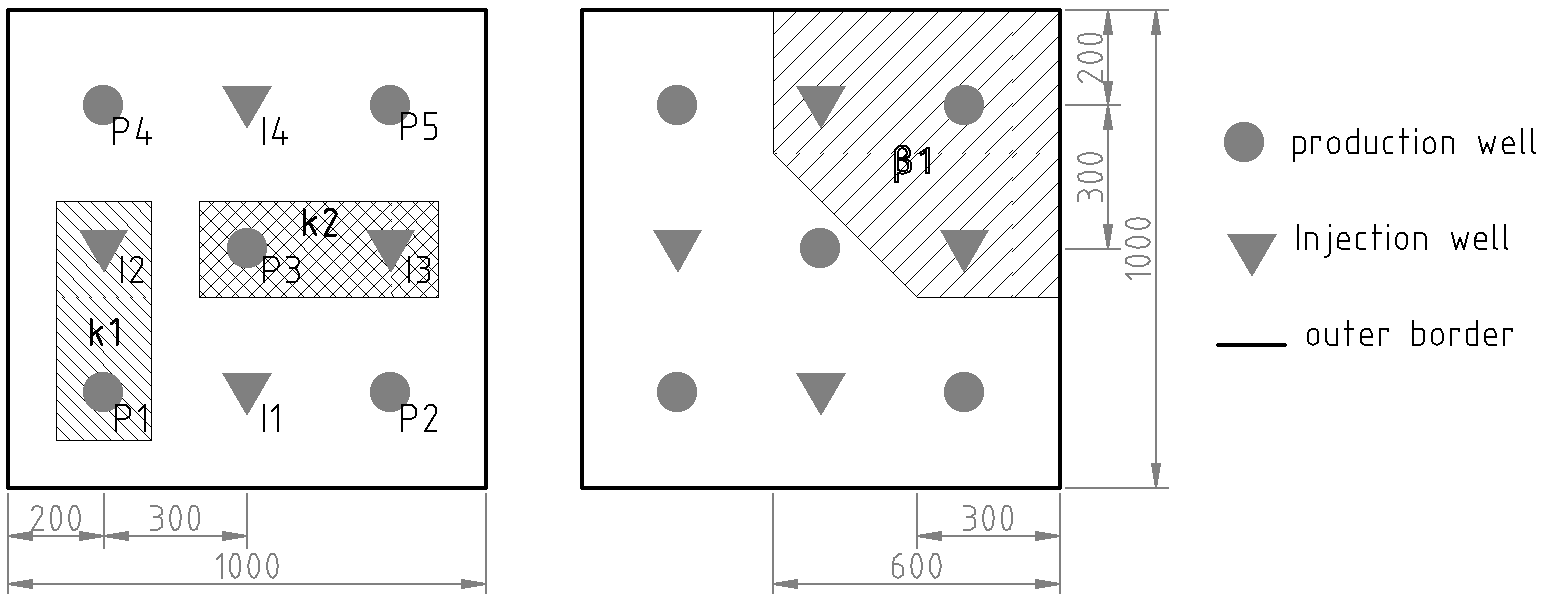
\includegraphics[width=0.7\linewidth]{fig1}
	\caption{Схематичечское представление расчётной области Schematic representation of the computational domain spacing pattern}
	\label{fig:schime}
\end{figure}

В качестве источника исходных данных была использована синтетическая гидродинамическая модель. Набор данных получен путем прямого численного моделирования двухфазной фильтрации. Полученные данные были использованы для решения задачи адаптации и прогнозирования.
При решении обратной задачи в качестве режимов работы использованы дебиты добывающих скважин и приемистости нагнетательных скважин, полученные из прямого численного моделирования. Пористость, толщина пласта, начальные и граничные условия соответствовали прямой задаче. Обратная задача решается в оптимизационной постановке, в которой минимизируется целевая функция {\ref{mse}}. В качестве фактических замеров пластового давления использовалось ограниченное количество давлений, полученные из решения прямой задачи. Случайным образом выбраны 10\% от общего количества значений пластового давления, которые выступали в качестве истинных значений.

Период моделирования составлял 10 лет, на протяжении которых скважины работали с заданными режимами. Расчетный шаг составлял 1 месяц. Зависимости приемистости нагнетательных скважин от времени, приведенные на рис. \ref{inj_rate}, получены путем случайной генерации и имеют кусочно-постоянный вид. Так же с заданной периодичностью происходит отключение нагнетательных скважин, период простоя составлял от 2 до 4 месяцев. На добывающих скважинах заданы изменяющиеся по гармоническому закону забойные давления, которые приведены на рис. \ref{prod_rate}.

Полученный набор данных был использован для решения обратной задачи. При этом для оценки прогностических свойств модели данные были разделены на обучающую и тестовую выборки. Первые 7 лет истории разработки отнесены к обучающей выборке и использованы для адаптации модели. Период 7-10 лет включен в тестовую выборку для которой проведены прогнозные расчеты. 

\begin{figure}
	\centering
	\begin{minipage}{0.5\linewidth}
		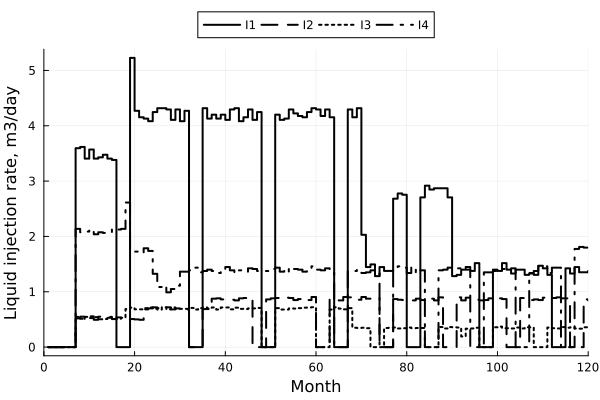
\includegraphics[width=1\textwidth]{fig2}
		\caption{a}
		\label{inj_rate}
	\end{minipage}%
	\begin{minipage}{0.5\linewidth}
		\centering
		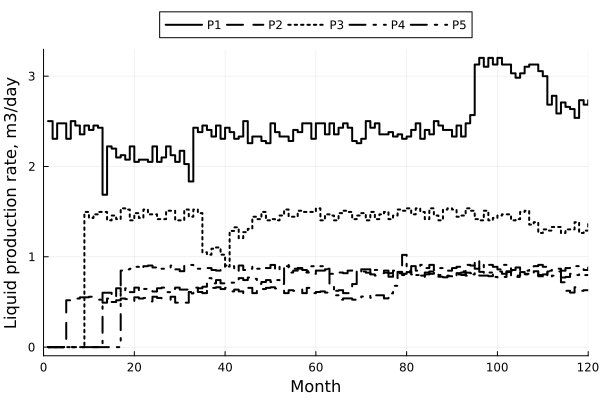
\includegraphics[width=1\textwidth]{fig3}
		\caption{b}
		\label{prod_rate}
	\end{minipage}
	\caption{Динамика приемистости нагнетательных скважин I1-I4 Injectivity dynamics of injection wells I1-I4}
\end{figure}

 Начальное пластовое давление составляло 20 МПа. На границах элемента разработки задано Постоянное пластовое давление $Pa = 20 МПа$. Параметры горной породы и насыщающих ее флюидов, принятые для расчета, имели следующие значения: пористость 0.2, значения абсолютной проницаемости представлены в виде карты на рис. 1, эффективная вязкость 1 мПа*c. Толщина пласта принята равной 4 м.

Решение оптимизационной задачи осуществляется встроенными в пакет Flux оптимизационными алгоритмами (Descent и ADAM). В результате решения были получены карты подвижности \ref{fig:mob} и карты эффективной сжимаемости \ref{comp}. Несмотря на отличия, видно, что поля качественно повторяют исходные (\ref{fig:schime}). Кроме поля подвижности в \ref{tabl:connection} представлены значения связей между скважинами, которые были получены методом частичного исключения переменных из численной фильтрационной модели \cite{and}. Наибольшие значения связей I2-P1 и I3-P3 соответствуют зонам с высокими значениями проницаемости (каналам). Коэффициенты связей имеют смысл проводимости между скважинами на единицу толщины пласта. Подобные коэффициенты связи могут быть получены при интерпретации попарного гидропрослушивания скважин.

\begin{figure}
	\centering
	\begin{minipage}{0.5\linewidth}
		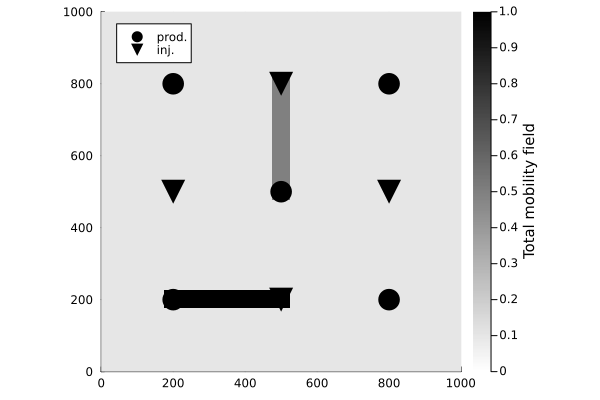
\includegraphics[width=1\textwidth]{fig4}
		\caption{a}
		\label{fig:mob}
	\end{minipage}%
	\begin{minipage}{0.5\linewidth}
		\centering
		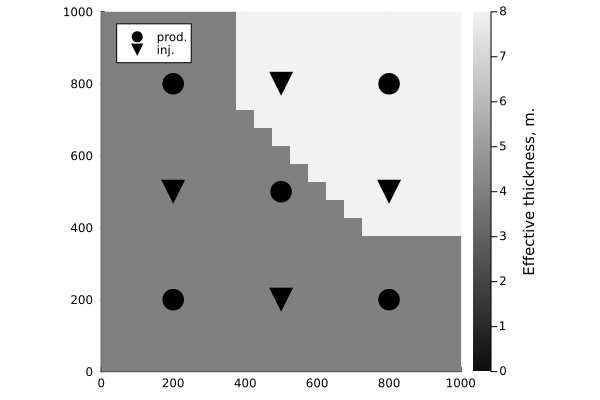
\includegraphics[width=1\textwidth]{fig5}
		\caption{b}
		\label{comp}
	\end{minipage}
	\caption{a Поле общей подвижности на конце обучающей выборки Total mobility field at the end of the training set
	b Восстановленное поле общей подвижности Restored general total field}
\end{figure}

 На основе рассчитанных для величин связей между скважинами выполнено количественное сопоставление истинного и восстановленного поля общей подвижности. Сравнение основных связей приведено в таблице \ref{tabl:connection} из которой видно, что ранжирование восстановленных связей полностью совпадает с ранжированием истинных связей. Кроме того, получено удовлетворительное количественное совпадение величин связей: в среднем относительная ошибка составляет 9\%. Таким образом, восстановленное поле общей подвижности качественно и количественно воспроизводит ключевые особенности истинного поля.

\begin{figure}
	\centering
	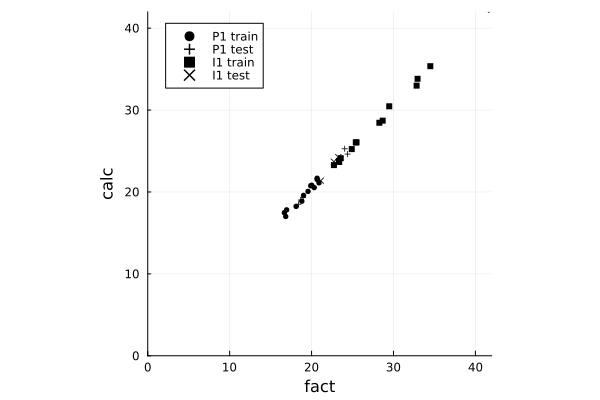
\includegraphics[width=0.7\linewidth]{fig6}
	\caption{Сопоставление фактических и расчетных значений пластового давления для добывающих и нагнетательных скважин. Полые маркеры соответствуют обучающей выборке, закрашенные – тестовой выборке. Пунктирная линия обозначает интервал отклонения в 10\% Comparison of true and calculated values of reservoir pressure for production and injection wells. Hollow markers correspond to the training set, filled markers correspond to the test set. The dotted line indicates the 10\% deviation interval}
	\label{fig:cp}
\end{figure}


Количественное сопоставление истинных и оценочных значений эффективной сжимаемости представлено на рисунке 8. На рисунке столбцы 1 и 2 соответствуют истинным и оценочным значениям. Значения были получены путем усреднения значений, полученных из карты, и входящих в соответствующий полигон Вороного для соответствующей скважины. 


Для реальных пластовых систем величины связей между скважинами, как правило, достоверно не известны. В виду этого одним из основных критерием для оценки качества адаптации модели выступают замеры пластового давления. На рис. \ref{fig:cp} приведено сравнение значений фактических и расчетных давлений для пары скважин I1, P1, полученных после восстановления поля общей подвижности и эффективной сжимаемости. На рисунке разными маркерами обозначены значения соответствующей обучающей (train) и тестовой (test) выборкам. Получено удовлетворительное совпадение давлений на обучающей и тестовой выборке, значения средней относительной ошибки для которых составляет 3.6 и 5.5\% соответственно. Модель демонстрирует удовлетворительную точность на тестовой выборке, что подтверждает ее прогнозные свойства.


	\begin{table}[h!]
	\caption{Коэффициенты связей между скважинами}	
	\label{tabl:connection}	
	\begin{center}
		\begin{tabular}{c|c|c|c|c}
			\hline
			Связь & Истинное значение & Восстановленное значение & Относительная ошибка д.ед. \\
			\hline
				I2-P1 & 20.6 & 20.6 & 0.1 \\ 
				I3-P3 & 5.51 & 5.51 & 0.1 \\ 
				P3-I2 & 0.488 & 0.488 & 0.1 \\ 
				I1-P1 & 0.338 & 0.338 & 0.1 \\ 
				I4-P3 & 0.297 & 0.297 & 0.1 \\ 
				P3-I1 & 0.296 & 0.296 & 0.1 \\ 
				P5-I3 & 0.295 & 0.295 & 0.1 \\ 
			\hline
			
		\end{tabular}
	\end{center}
\end{table}


\section{CONCLUSIONS}

Представлен подход к совместному использованию теории фильтрации и машинного обучения для решения задачи адаптации модели на исторические данные. На примере синтетической модели элемента нефтяного месторождения с регионально неоднородным полем проницаемости и эффективной сжимаемостью была продемонстрирована реализация этого подхода. Адаптация модели однофазной фильтрации к историческим данным была достигнута путем восстановления полей проницаемости и эффективной сжимаемости с использованием сети радиальных базисных функций и полносвязного линейного слоя. На основе реконструированного поля подвижности рассчитываются коэффициенты связи между скважинами, которые количественно соответствуют истинным связям в системе. На основе рассчитанного поля упругоёмкости методом осреднения получены средние значения показателей упругоёмкости вблизи скважин, которые также качественно совпадают с исходными. Таким образом, предлагаемый подход позволяет восстановить характерный вид зональной неоднородности моделируемого объекта. Универсальный вид предлагаемого подхода предполагает возможность использования более сложных видов моделей машинного обучения.

\section{FUNDING}
«Исследование выполнено за счет гранта Российского научного фонда № 24-21-00468,
 https://rscf.ru/project/24-21-00468/»
 
 \begin{thebibliography}{20}
	
\bibitem{mus1} E. N. Musakaev, S. P. Rodionov and N. G. Musakaev, "Hierarchical Approach to Identifying Fluid Flow Models in a Heterogeneous Porous Medium," Mathematics, 9(24), 3289 (2021).

\bibitem{bek} A. D. Bekman, T. A. Pospelova and D. V. Zelenin,  "A new approach to water cut forecasting based on results of capacitance resistance modeling" Vestn. Tyumen. Univ., Fiz. Mat. Model. Neft’, Gaz, Energet. 6 (1(21)), 192–207 (2020).

\bibitem{pot} K.A. Potashev, R.R. Akhunov and  A.B. Mazo, "Calculation of the flow rate between wells in the flow model of an oil reservoir using streamlines", Georesources. 24(1), 27–35 (2022).

\bibitem{tem}  P. Temirchev, M. Simonov, R. Kostoev, E. Burnaev, I. Oseledets, A. Akhmetov, A. Margarit, A. Sitnikov and D. Koroteev, "Deep neural networks predicting oil movement in a development unit", Journal of Petroleum Science and Engineering. 184. 106513 (2020).

\bibitem{uma} A. W. Umanovskiy, "Proxy modeling pf reservoir hydrodynamics with graph neural networks",Vestn. Tyumen. Univ., Fiz. Mat. Model. Neft’, Gaz, Energet. 8 (3(31)), 155-177 (2022).

\bibitem{kos2} V. P. Kosyakov and D. Yu. Legostaev, “Using elements of machine learning to solve the inverse problem of reconstructing the hydraulic conductivity feld for a fltration problem,” Vestn. Tyumen. Univ., Fiz. Mat. Model. Neft’, Gaz, Energet. 8 (2 (30)), 129–149 (2022).

\bibitem{kos3} V.P.Kosyakov, S.P.Rodionov, "Optimal control of wells on the basis of two-phase filtration equations",  Tr. MFTI. 8(3), 79-90 (2016).

\bibitem{far} P. E. Farrell, D. A. Ham, S. W. Funke and M. E. Rognes, "Automated Derivation of the Adjoint of High-Level Transient Finite Element Programs",SIAM Journal on Scientific Computing, 35(4) 369-393 (2013).

\bibitem{inn}  M. Innes, E. Saba, K. Fischer, D. Gandhi, M. C. Rudilosso, N. M. Joy, T. Karmali, A. Pal and V. B. Shah, "Fashionable Modelling with Flux", ArXiv. 1811.01457 (2018).

\bibitem{and} V. B. Andreev, \textit{Numerical methods}. (М.: MAKS Press)[in Russian].

\bibitem{azi} H. Aziz, E. Settari. \textit{Mathematical modeling of reservoir systems}.  M.-Izhevsk: Institute for Computer Research, 2004. [in Russian]


\end{thebibliography}

\end{document}
